\documentclass[a4paper,12pt]{article} % A4, шрифт 12pt
\usepackage[left=30mm, right=15mm, top=20mm, bottom=20mm]{geometry} % Поля
\usepackage{setspace}  % Для изменения межстрочного интервала
\onehalfspacing  % Межстрочный интервал 1.5
\usepackage{indentfirst}  % Красная строка в первом абзаце секции
\setlength{\parindent}{1.25cm}  % Абзацный отступ 1.25 см


\usepackage[T2A]{fontenc}			
\usepackage[utf8]{inputenc}			
\usepackage[english,russian]{babel}	

\usepackage{amsmath,amsfonts,amssymb,amsthm,mathrsfs,mathtools} 
\usepackage{cancel}
\usepackage{multirow}
\usepackage[colorlinks, linkcolor = blue]{hyperref}
\usepackage{upgreek}
\usepackage{graphicx,wrapfig}
\usepackage{bm}
\usepackage{float}
\usepackage[table]{xcolor} % убран xcdraw
\usepackage{tikz}
\usepackage{pgfplots}
\graphicspath{{pictures/}}

\usepackage[sorting=none,backend=biber,style=gost-numeric]{biblatex}
\addbibresource{references.bib}


\usepackage{graphicx}
\usepackage{subcaption}

\usepackage[acronym]{glossaries}

\makeglossaries


\newacronym{abm}{ABM}{Agent-based model (от англ. агентная модель)}

\newacronym{sir}{SIR}{susceptible $\rightarrow$ infectious $\rightarrow$ recovered (от англ. восприимчивый $\rightarrow$ инфицированный $\rightarrow$ восстановившийся)}

\newacronym{sirp}{SIRP}{susceptible $\rightarrow$ infectious $\rightarrow$ recovered $\rightarrow$ partially immune (от англ. восприимчивый $\rightarrow$ инфицированный $\rightarrow$ восстановившийся $\rightarrow$ частично иммунный)}

\newacronym{sis}{SIS}{susceptible $\rightarrow$ infectious $\rightarrow$ susceptible (от англ. восприимчивый $\rightarrow$ инфицированный $\rightarrow$ восприимчивый)}

\newacronym{seir}{SEIR}{susceptible $\rightarrow$ exposed $\rightarrow$ infectious $\rightarrow$ recovered (от англ. восприимчивый $\rightarrow$ подверженный $\rightarrow$ инфицированный $\rightarrow$ восстановившийся)}

\newacronym{seis}{SEIS}{susceptible $\rightarrow$ exposed $\rightarrow$ infectious $\rightarrow$ susceptible (от англ. восприимчивый $\rightarrow$ подверженный $\rightarrow$ инфицированный $\rightarrow$ восприимчивый)}

\newacronym{siqs}{SIQS}{susceptible $\rightarrow$ infectious $\rightarrow$ quarantined $\rightarrow$ susceptible (от англ. восприимчивый $\rightarrow$ инфицированный $\rightarrow$ изолированный $\rightarrow$ восприимчивый)}

\newacronym{zppp}{ЗППП}{заболевания, передающиеся половым путем}

\newacronym{mp}{MP}{message passing (от англ. обмен сообщениями)}

\newacronym{ebcm}{EBCM}{edge-based compartmental models (от англ. компартментные модели на ребрах графа)}

\newacronym{covasim}{Covasim}{COVID-19 Agent-based Simulator}

\newacronym{covid}{COVID-19}{Coronavirus Disease 2019}

\newacronym{anova-hdmr}{ANOVA-HDMR}{ANalysis Of VAriance high-dimensional model representation (от англ. анализ дисперсии по многомерному представлению)}


\begin{document}

\begin{titlepage}

\begin{center}
    {\large Министерство образования и науки Российской Федерации}
\end{center}
\begin{center}
    {\large Федеральное государственное автономное 
образовательное учреждение высшего образования 
«Московский физико-технический институт 
(государственный университет)»}
\end{center}
\begin{center}
    {\large Физтех-школа биологической и медицинской физики \\ Кафедра системной и синтетической биологии}
\end{center}

    \vspace{3.5cm}


\vspace{0.1cm}
{\huge
\begin{center}
    \textbf{Исследование роли транспортных потоков в развитии эпидемии на основе компьютерной агентной модели}
   \\
\end{center}
}
{\large
\begin{center}
    Выпускная квалификационная работа бакалавра
   \\
\end{center}
}

\vspace{3.5cm}

\begin{flushright}
\large Выполнил:\\ студент Б06-101 группы, \\Клочков Константин Александрович.
\vspace{0.2cm}
\end{flushright}

\begin{flushright}
\large Научный руководитель: \\ к.б.н, Манолов Александр Иванович.
\vspace{0.2cm}
\end{flushright}

\vspace{2.5cm}

\begin{center}
    Долгопрудный, 2025
\end{center}

\end{titlepage}


\tableofcontents
\newpage
\section{Список сокращений}



\printacronyms
\newpage
\section{Введение}

\newpage
\section{Обзор литературы}
\subsection{Виды эпидемиологических моделей}

Математические модели стали важными инструментами анализа распространения инфекционных заболеваний и способов борьбы с ними. В процессе создания модели уточняются предположения и параметры, а само моделирование позволяет оценить критические значения параметров модели, приводящие к развитию эпидемии, индекс репродукции инфекции $R_0$, среднее число контактов между людьми $\sigma$. Математические модели и компьютерное моделирование являются полезными экспериментальными инструментами для проверки теорий, оценки количественных гипотез, ответов на конкретные вопросы, определения чувствительности к изменениям значений параметров и оценки ключевых параметров по данным. Понимание особенностей передачи инфекционных заболеваний в сообществах, регионах и странах может привести к улучшению подходов к снижению распространения этих заболеваний. Математические модели используются при сравнении, планировании, реализации, оценке и оптимизации различных методов
программ по выявлению, профилактике, лечению и контролю. Моделирование в эпидемиологии может способствовать разработке и анализу эпидемиологических обследований, предлагать важнейшие данные которые необходимо собрать, выявить тенденции, сделать общие прогнозы и оценить неопределенность прогнозов \cite{hethcote2000mathematics, hethcote1989three,hethcote1992transmission}.

\subsubsection{Детерминистические компартментные модели}

Подавляющее большинство эпидемиологических моделей основано на компартментализации людей в зависимости от их состояния \cite{keeling2005networks,kermack1927contribution,bailey1957mathematical,anderson1992may}. Базовые модели описывают лишь три компартмента: восприимчивых, инфицированных и восстановившихся. В таком случае происходит пренебрежение многими деталями развития эпидемии, тем не менее такие модели все еще активно применяются. Основным из используемых типов является \gls{sir} модель, описываемая системой дифференциальных уравнений
\begin{equation}
    \left\{
    \begin{aligned}
    & \frac{dS}{dt}=bN-\lambda S-dS, \\
    & \frac{dI}{dt}=\lambda S-gI-dI, \\
    & \frac{dR}{dt}=gI-dR,
    \end{aligned}
    \right.
\end{equation}
и \gls{sis} модель
\begin{equation}
    \left\{
    \begin{aligned}
        & \frac{dS}{dt} = gI-\lambda S, \\
        & \frac{dI}{dt} = \lambda S - gI.
    \end{aligned}
    \right.
\end{equation}

Переменные $S$, $I$, $R$ обозначают количества восприимчивых, инфицированных, восстановившихся людей соответственно; $N$ --- размер популяции; $b$, $d$, $g$ --- коэффициенты рождаемости, смертности и восстановления (доля рождающихся, умирающих, восстанавливающихся людей в единицу времени); $\lambda$ --- сила инфекции (доля восприимчивых людей, инфицируемых в единицу времени).

\gls{sir} модели применяются для описания инфекционных заболеваний, формирующих очень стойкий или пожизненный иммунитет, например, кори, коклюша \cite{keeling2005networks,kermack1927contribution,anderson1992may,grenfell1992chance,rohani2000impact}. \gls{sis} модели используют преимущественно при описании распространения \glslink{zppp}{\glsentryshort{zppp}}, реинфицирование которыми вполне возможно, например, хламидиоза, гонореи \cite{keeling2005networks,hethcote1984springer,garnett1996sexually}.

Также активно применяются модифицированные модели с уточненной компартментализацией для более сложного протекания болезни \cite{keeling2005networks, anderson1988epidemiology, grenfell2001travelling} и с более проработанной структурой популяции \cite{hethcote1984springer, ghani1997role, keeling1997modelling}.


\begin{figure}[]
    \centering
    \begin{subfigure}{0.45\linewidth}
        \centering
        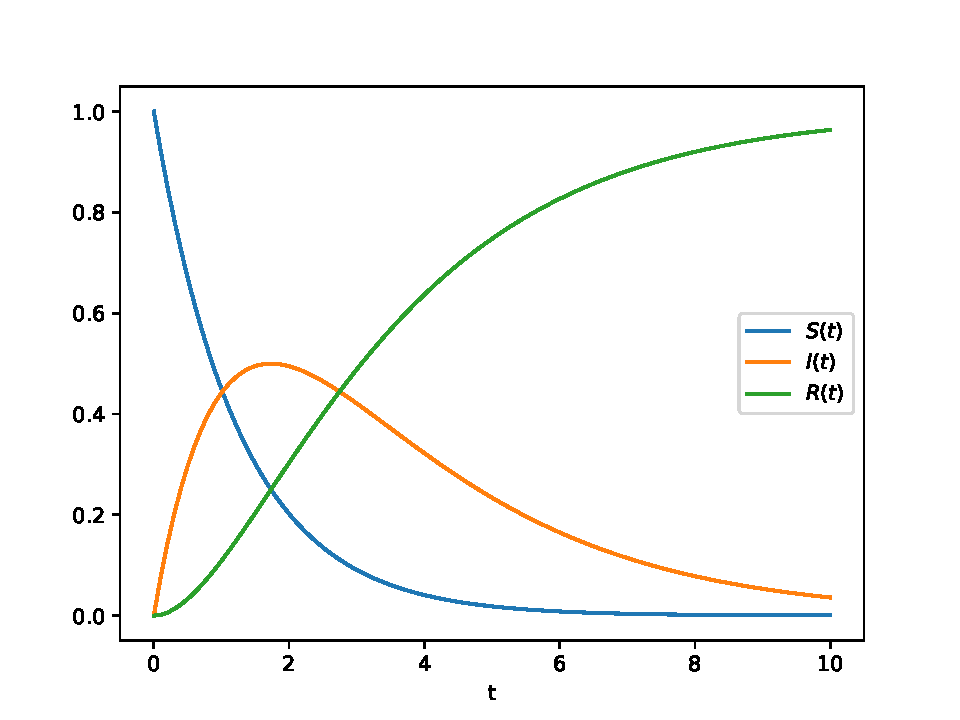
\includegraphics[width=\linewidth]{images/sir.pdf}
        \caption{\gls{sir} модель}
    \end{subfigure}
    \hfill
    \begin{subfigure}{0.45\linewidth}
        \centering
        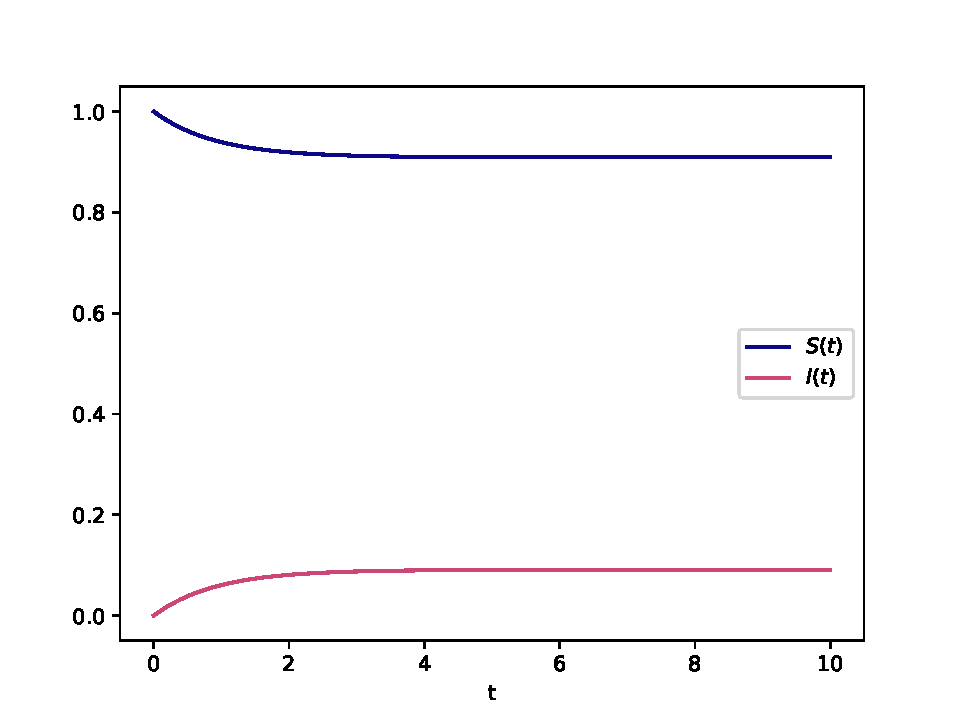
\includegraphics[width=\linewidth]{images/sis.pdf}
        \caption{\gls{sis} модель}
    \end{subfigure}
    \caption{Численные решения задачи Коши компартментных моделей с начальными условиями $S(0)=1$, $I(0)=0$, $R(0)=0$ и параметрами $b=d=0$, $g=0.4$, $\lambda=0.8$, $N=1$}
\end{figure}

\subsubsection{Детерминистические модели среднего поля}
Компартментные модели строятся в предположении, что каждый человек взаимодействует с каждым. На самом деле в большой популяции у каждого индивида есть свой ограниченный круг общения, и именно им определяется путь распространения инфекции, причем число контактов очень сильно меняется от человека к человеку \cite{pastor2001epidemic}. Для более реалистичного описания таких социальных взаимодействий распространение эпидемии моделируют на графе контактов (или сети контактов), в котором каждому человеку соответствует узел, а каждой социальной связи --- ребро графа \cite{sherborne2018mean}.

В связи с тем, что прямой анализ стохастического поведения эпидемии на графе является сложным, его описывают детерминистическим приближением среднего поля, анализируя некоторые характерные средние характеристики моделей \cite{sherborne2018mean}. Другими словами, в таких моделях для упрощения математического описания вводятся различные приближения: попарные модели рассматривают состояния пар узлов, соединенных ребром \cite{keeling1999effects, house2011insights}; \gls{mp} модели рассматривают каждый узел и все возможные пути передачи инфекции в этот узел независимо \cite{karrer2010message}; модели средней степени вершины графа учитывают звездчатые структуры --- узлы с их соседями с учетом их состояния \cite{lindquist2011effective}; \gls{ebcm} оценивают вероятность случайного узла остаться восприимчивым \cite{miller2012edge}. Все эти модели можно построить на одном и том же графе контактов, исходя из разных предположений, но, на самом деле, часть из них оказывается эквивалентна друг другу \cite{sherborne2018mean}.

Эти модели лучше описывают социальное устройство популяции, однако они рассматривают марковский процесс, то есть исходят из предположения, что состояние графа на следующем шаге определяется лишь его состоянием на текущем шаге и никак не зависит от предыдущих шагов. Эти предположения часто оказываются неверны, так как инфицирование или выздоровление происходит не случайно в любой момент времени, а после конкретного инкубационного периода или периода болезни соответственно \cite{keeling2005networks,volz2008sir,house2011insights}. 

\subsubsection{Стохастические модели}
Результатами применения стохастических моделей также являются временные зависимости некоторых глобальных величин \cite{aiello2003new,haas1999temporal}, однако, в отличие от детерминистических моделей, стохастический подход допускает временные флуктуации как на глобальном уровне, так и на локальном --- флуктуации на уровне агентов в зависимости от их контактов \cite{nakamura2017efficient}.

Основой таких моделей, как и с моделями среднего поля, часто является граф взаимодействий, часто описываемый матрицей контактов $A$ \cite{albert2002statistical}. В отличие от компартментных моделей, матрица контактов может содержать в себе крайне сложные социальные структуры, что позволяет наблюдать более широкий спектр эпидемиологических явлений \cite{pastor2015epidemic}. Распространение инфекции задается матрицей перехода $\hat{T}$, матричные элементы $T_{\mu\nu}$ которой равны вероятностям перехода из состояния графа $\nu$ в $\mu$ \cite{van1992stochastic}. Эта разница между компартментными и стохастическими моделями приводит к различию между временными зависимостями эпидемиологических статистик. К примеру, оказывается, что, хоть \gls{sis} модель демонстрирует схожее с аналогичной стохастической поведение при различных соотношениях между силой инфекции и коэффициентом восстановления, на ранних этапах развития эпидемии, когда среднее число инфицированных сильно меньше размера популяции, ключевым фактором являются именно флуктуации числа инфицированных. И именно такому режиму соответствуют санитарные меры по сдерживанию эпидемий на ранних стадиях \cite{nakamura2017efficient}.

\subsubsection{Агентные модели}
\gls{abm} применяются при моделировании распространения инфекционных заболеваний уже более 40 лет \cite{fox1971herd, elveback1976influmza}, однако из-за недостатка данных и вычислительных мощностей раскрывать свой потенциал они начали совсем недавно \cite{koopman2002controlling}.

Устройство \gls{abm} позволяет напрямую описывать сложные социальные и физические системы. Хоть для воспроизведения социальной структуры конкретной страны или города может потребоваться очень много данных, \gls{abm} может отразить неоднородность социальных взаимодействий и динамические изменения в структуре сети \cite{rakowski2010influenza}. 

Такой подход очень полезен для простой реализации учета иммунологической истории индивидов, вариации климата между регионами, социальных структур, что позволяет проводить более тонкую калибровку. Также \gls{abm} позволяют рассматривать распространение инфекции в маленьких группах людей \cite{rakowski2010influenza}.

Построение \gls{abm} требует, во-первых, воссоздания искусственной популяции, соответствующей демографическим данным в регионе, и, во-вторых, создания сети публичных объектов, таких как школ, рабочих мест, где агенты могут взаимодействовать друг с другом. Главной сложностью при построении \gls{abm} является тот факт, что требуемая информация часто скрыта при агрегировании федеральными службами государственной статистики. В связи с этим возникает необходимость в разработке методов, позволяющих воссоздать исходные данные из агрегатов, или моделей, приближающих искомые данные \cite{rakowski2010influenza}. 

\subsection{Подходы к изучению транспортных потоков в эпидемиологии}
Транспорт играет важнейшую роль в жизни людей и в то же время активно способствует распространению эпидемий. В связи с этим введение ограничений на транспортные потоки является важной эпидемиологической мерой \cite{li2021modeling}, а понимание влияния этих мер позволит человечеству эффективнее бороться с распространением инфекционных заболеваний.

В имеющихся исследованиях по этой теме транспорт описывается преимущественно математическими моделями, моделями на графах и агентными моделями. Статистические (регрессионные и авторегрессионные модели на пространственных данных) же для этих целей практически не применяются в связи с необходимостью иметь огромное множество данных о мобильности людей, в отсутствие которых качество результатов работы таких моделей крайне ограничено. Клеточными автоматами симулировать перемещение индивидов также затруднительно, так что их для этих целей тоже применяют редко \cite{li2021modeling}.

\subsubsection{Математические модели}
Одним из преимуществ математических моделей является тот факт, что для их калибровки требуются малые объемы данных. По этой причине было предпринято множество попыток адаптирования существующих математических моделей под описание системы нескольких городов. Хоть эти модели и предполагают, что города обладают одинаковыми демографическими параметрами, что перемещения происходят мгновенно, некоторые игнорируют возможность инфицирования при перемещении, из них можно получить важные выводы \cite{li2021modeling}.

Дж. Хайман и др. (2003) \cite{hyman2003modeling} для описания распространения гриппа в США в присутствие авиатранспорта каждый исследуемый город описали моделью типа \gls{sirp} --- добавили компартмент, содержащий частично имунных агентов, в который попадает часть восстановившихся. Перемещения людей ввели, определив постоянную матрицу миграции $M$, содержащую долю перемещающихся людей в единицу времени, внеся в производные $\frac{d}{dt}(S_k,I_k,R_k,P_k)$ слагаемое $\sum\limits_{j=1}^n \left[m_{jk}\frac{(S_j,I_j,R_j,P_j)}{N_j}-m_{kj}\frac{(S_k,I_k,R_k,P_k)}{N_k}\right]$. В результате авторы выявили, что наиболее эффективно замедляет эпидемию сокращение продолжительности инфекционной стадии, сокращение числа контактов $r$, уменьшение вероятности передачи $\beta$. Этот подход полностью игнорирует возможность инфицирования при перемещении, что некорректно особенно при рассмотрении быстро распространяющихся заболеваний как грипп или атипичная пневмония, ведь во время поездок люди в течение долгого времени находятся в очень близком контакте друг с другом \cite{li2021modeling}.

Ванг и Жао (2004) \cite{wang2004epidemic} на совокупности \gls{sis} на двух примерах проиллюстрировали важность перемещения агентов в развитии эпидемии: первый показал, что при большом индексе репродукции инфекции одного города пассажиропотоки могут усилить распространение болезни, если же пассажиропотоки большие при малых числах репродукции во всех населенных пунктах, то наличие транспорта может снизить распространение. Второй пример продемонстрировал, что инфекция из-за транспортных потоков может стать эндемичной, даже если в каждом изолированном городе она должна исчезнуть.

Такеучи и др. (2006) \cite{takeuchi2006spreading} предложили аналогичный подход для системы из двух \gls{sis} и ввели слагаемое, учитывающее инфицирование агентов в процессе перемещения между населенными пунктами, считая, что частота заболевания туристов $\gamma(\alpha S_j)(\alpha I_j)/(\alpha S_j+\alpha I_j)$, где $\gamma$ --- трансмиссивность инфекции в процессе перемещения, $\alpha$ --- доля перемещающихся агентов в единицу времени. Анализ этой \gls{sis} привел авторов к выводу, что инфицирования, связанные с транспортными потоками, приводят к повышению как абсолютного, так и относительного числа больных, что подтверждает необходимость вводить транспортные ограничения сразу при обнаружении вспышки инфекции \cite{takeuchi2006spreading}.

Лиу и Такеучи (2006) \cite{liu2006spread} рассматривали возможность тестирования инфицированных агентов и помещения их в карантинный компартмент в системе двух \gls{siqs}, учитывая туризм аналогично авторам упомянутым выше. Они пришли к тому, что входной скрининг с последующим карантином инфицированных крайне полезен, так как всегда может привести к завершению эпидемии, даже если инфекция эндемична в каждом из рассматриваемых городов \cite{liu2006spread}.

Ван и Цуй (2007) \cite{wan2007seis} исследовали возможности контроля распространения инфекционных заболеваний, изучая модель \gls{seis}. Оказалось, что даже если запретить инфекционным агентам перемещаться, инфицированные в инкубационной фазе все равно приносят болезнь в города.                                                                                                                                                                                                                                                                                                                          Помимо этого они подтвердили результаты, полученные ранее Вангом и Жао \cite{wang2004epidemic} и Такеучи и др. \cite{takeuchi2006spreading}, о том, что наличие транспортных потоков может качественно изменить ход эпидемии.

Лиу и Жоу (2007) \cite{liu2009global} при анализе \gls{sir} вывели, что при базовом репродуктивном числе $R_{0_\gamma} \leqslant 1$ болезнь исчезает со временем, и это состояние глобально асимптотически устойчиво. Если же $R_{0_\gamma} > 1$ существует локально асимптотически устойчивое эндемическое равновесие, то есть болезнь остается в популяции. Также, как и у Ванг и Жао \cite{wang2004epidemic}, авторы получили, что при наличии транспорта инфекция может стать эндемичной, даже если в каждом отдельном городе в отсутствие перемещений агентов она должна была исчезнуть. Аналогичный результат получили и Ли и Жоу (2009) \cite{li2010dynamics}, используя систему дифференциальных уравнений с запаздыванием при учете латентного периода в \gls{sir}.

\subsubsection{Модели на графах}
\subsubsection{Агентные модели}
В \gls{abm} каждому агенту могут быть присвоены свои аттрибуты, при этом каждый принимает индивидуальные решения, что позволяет отразить все детали межличностных взаимодействий. В связи с развитием систем общественного транспорта им пользуется все больше людей, что значительно усложняет сеть контактов. Поэтому моделирование транспортных систем очень важно в эпидемиологических \gls{abm}.

Симоэс (2006) \cite{simoes2006modelling} для описания эпидемии паротита в Португалии 1996 года разработала \gls{abm}, состоящую из \gls{seir} и транспортной модели: она базировалась на делении Португалии на регионы, между которыми вводились 4 типа перемещений, связанные с различными типами социальных активностей: движения в пределах квартала; региона; между соседними регионами и между удаленными регионами. Перемещение агента на каждом шаге по времени определялось взвешенной суммой всевозможных перемещений между регионами с весами, равными вероятностям этих перемещений. Такой подход учитывает пространственное распределение популяции и ее перемещения, что позволило получить результаты моделирования эпидемии паротита близкие к реальным.

Раковски и др. (2010) \cite{rakowski2010influenza} при построении \gls{abm} распространения гриппа в Польше использовали простые правила транспортировки для имитации поездок людей и позволили в модели инфекции передаваться непосредственно в транспорте. Авторы выбрали 38 крупнейших городов Польши и на основе их построили граф транспортной сети, в котором веса ребер были пропорциональны расстоянию между городами и обратно пропорциональны размерам их популяций. С помощью алгоритма Дейкстры находился кратчайший маршрут между любыми двумя городами, а список промежуточных городов на этом пути заносился в матрицу $S$. На каждом шаге модели выбирались случайные агенты, отправляемые в другой город; каждому агенту назначался город прибытия (вероятность выбора города пропорциональна его населению); определялись города, в которых делались пересадки; формировались группы путешественников размером до 10 человек. Эта модель, хоть и не учитывает точные маршруты, позволяет оценить их исключительно из карты распределения плотности населения, что сильно снижает требования к объемам необходимых для моделирования данных.

Фриас-Мартинез и др. (2011) \cite{frias2011agent} первыми использовали реальные данные сотовых операторов в \gls{abm} для решения задачи моделирования транспортных потоков, ранее применялись только результаты опросов и переписей населения, которые не дают требуемого временного разрешения. Они оценили покрытия вышек операторов сотовой связи и на основе имеющихся данных создали модель перемещения пользователей, которая оценивала положение людей в каждый момент времени, и модель социальных связей, которая определяла наиболее близкие взаимоотношения. Помимо этого каждый агент подчинялся модели заболевания \gls{seir}. Так авторы выяснили, что ограничение на передвижение людей в 2009 году в Мексике позволило снизить пиковое число зараженных H1N1 гриппом на 10\% и отложить момент наступления этого пика на 2 дня.


Крукс и др. (2014) \cite{crooks2014agent} моделировали вспышки холеры в лагере для беженцев Дадааб в Кении с помощью \gls{abm}. Распорядок дня беженцев была внесена в поведение агентов и могла исполняться в специализированных для этого местах: школе, религиозном центре, магазине и так далее. Для этого карта Дадааба была оцифрована и поделена на участки по видам возможной там деятельности. Также каждый агент отличался личными характеристиками (пол, возраст), социальными связями (размер семьи, круга общения), уровнем иммунитета (симптоматичный, асимптоматичный), целями и приоритетами. На каждом шаге днем агент принимает решение, остаться там, где он находится, или переместиться, чтобы закрыть свои потребности (в воде, еде, школе), а ночью возвращается домой. Само распространение холеры определяется \gls{seir}, где инфицированные могут быть как симптоматическими, так и асимптотическими, а само заражение происходит из источников воды, а источники воды становятся заразными после того, как туда попали фекалии инфицированных. Благодаря полученной модели авторы смогли рассмотреть два сценария развития холеры: радиально от источника загрязенной воды и через дождевые стоки, причем результаты качественно совпадают с реальными данными, например, для лагеря Дагахлей. Потенциально такая модель может стать частью системы раннего предупреждения вспышек холеры.




\subsection{Агентная модель Covasim}

В этой работе в дальнейшем речь будет идти о модели \gls{covasim} и ее модернизации. \gls{covasim} --- \gls{abm} с открытым кодом, содержащая информацию о возрастной структуре и размере популяции, реалистичную систему передачи инфекции в разных социальных слоях (домашние хозяйства, школы, рабочие места, случайные контакты и др.), течение болезни, зависящее от возраста, иммунитет, определяемый уровнем антител. Также в данной модели реализовано множество различных эпидемиологических мер: социального дистанцирования, ношения масок, вакцинирования, тестирования и других.

Каждый запуск \gls{covasim} состоит из нескольких этапов. Сначала создается объект симуляции и загружаются все необходимые параметры. Затем в соответствии с данными о распределении возрастов создаются агенты и объединяются в сети контактов, параметры которой берутся из демографических данных (например, средний размер семьи, число случайных контактов и др.). Затем в цикле на каждом шаге по времени: производится масштабирование популяции (если необходимо для повышения производительности); обновляются состояния агентов, в том числе связанные с развитием инфекции; инфицируются случайные агенты; применяются эпидемиологические меры, вычисляются вероятности дальнейшего инфицирования по сети контактов; вычисляются результирующие метрики.

В \gls{covasim} реализована довольно сложная модель протекания болезни, в которой каждый агент может пребывать в одном из 9 состояний: восприимчивый, подвергшийся воздействию (инфицированный, но пока не инфекционный), инфекционный (разделяется по тяжести симптомов на пресимптоматический, бессимптомный, легкий, тяжелый, критический), восстановившийся и умерший. Длительности нахождения в каждой фазе заболевания определяются для каждого агента отдельно из логнормального распределения с параметрами, взятыми из исследований \gls{covid} \cite{lauer2020incubation, du2020serial, nishiura2020serial, pung2020investigation, linton2020incubation, he2020temporal, wang2020clinical, chen2020clinical, verity2020estimates, wolfel2020virological}. Вероятности приобретения симптомов, развития тяжелой, критической фазы или смерти различны для агентов в зависимости от их возраста, и эти данные также взяты из исследований \gls{covid} \cite{chen2020clinical, wolfel2020virological, o2021age, baguelin2020report, ferguson2020impact}. В зависимости от слоя, которому принадлежит связь, вероятность передачи инфекции домножается на $0.05$ для домохозяйства, на $0.01$ для школ и рабочих мест, на $0.005$ для случайных контактов, что согласуется с литературными данными \cite{zhang2020changes, lader2006time}.

\begin{figure}[]
    \centering
    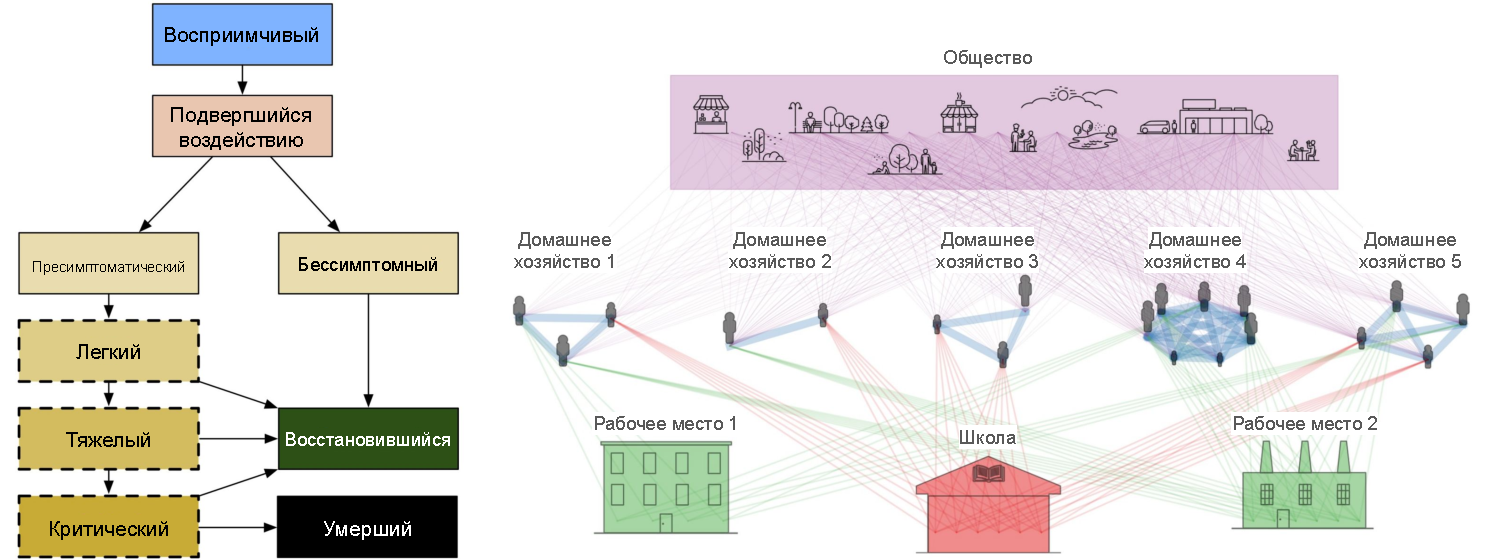
\includegraphics[width=\linewidth]{images/covasim.pdf}
    \caption{Структура модели развития инфекции (слева) и иллюстрация сети контактов в Covasim. Источник: \cite{kerr2021covasim}}
\end{figure}

В зависимости от объемов имеющихся демографических данных для запуска \gls{covasim} можно использовать 3 способа генерации синтетической популяции: случайные сети, SynthPops и гибридные сети.

В отсутствие данных применяются случайные сети: всем агентам из Пуассоновского распределения определяются числа контактов, после чего в соответствии с этими значениями формируются произвольные связи между людьми.

SynthPops применяется при наличии информации о вероятностях взаимодействий между возрастными группами в домохозяйствах, школах, на рабочих местах, на улице; о распределении численностей людей в школах, числах набора школьников разных возрастов, отношении числа преподавателей к числу школьников; о распределении численностей рабочих мест и числах трудоустроенных людей разных возрастов; о распределении размеров домохозяйств, возрастов и полов членов семей. 

При формировании связей в домохозяйствах SynthPops сначала выбирает размеры семей из их распределения, после чего за каждой семьей закрепляет главу семейства. Остальные члены домохозяйств набираются в соответствии с вероятностями контактов в семьях и распределением возрастов в них.

Контакты между учениками в школах формируются аналогично, собирая агентов по семьям (дети из одних домохозяйств в одних школах), после чего выбираются агенты-работники учебного заведения и в зависимости от размера школы либо создаются контакты между всеми школьниками и работниками, либо каждому работнику определяется число связей с учениками, которые затем формируются.

Связи на рабочих местах формируются аналогично из агентов случайных домохозяйств. Также после определения чисел случайных контактов они добавляются SynthPops.

Для создания гибридной сети необходимы данные о распределении возрастов и размеров семей, однако они уже загружены в \gls{covasim} для каждой страны. Гибридный подход не учитывает распределение возрастов в домохозяйствах, все дети (все агенты от 6 до 22 лет) объединяются в школы, взрослые (агенты возрастом между 22 и 65) в рабочие места с предопределенными для них числами контактов в этих слоях из Пуассоновских распределений. Это позволяет воссоздать некоторую популяционную гетерогенность в случае недостатка демографических данных.



\subsection{Дисперсионный анализ чувствительности математических моделей}

В данной работе анализ чувствительности модели будет проводиться с помощью дисперсионных методов в связи с её стохастичностью и их информативностью, несмотря на большие вычислительные затраты: такие методы никак не зависят от природы модели и позволяют оценить влияние изменений любых комбинаций параметров \cite{saltelli2008global}.

Пусть задана квадратично интегрируемая функция $f$ на $\Omega^k$, единичном k-мерном гиперкубе,
\begin{displaymath}
\Omega^k=(X|0\leq x_i \leq 1;i=1,\ldots ,k),
\end{displaymath}
Илья Меерович Соболь предложил раскладывать эту функцию в сумму по возрастающим размерностям:
\begin{displaymath}
f=f_0+\sum\limits_i f_i + \sum\limits_i \sum\limits_{j>i} f_{ij}+\ldots+f_{12\ldots k},
\end{displaymath}
где каждое слагаемое также является квадратично интегрируемым на области определения и является функцией лишь коэффициентов в его индексе, то есть $f_i=f_i(X_i)$, $f_{ij}=f_{ij}(X_i,X_j)$ и так далее. Соболь показал, что слагаемые суммы можно последовательно вычислить из результатов расчетов модели $Y$ как
\begin{align*}
&f_0=E(Y) \\
&f_i=E(Y|X_i)-E(Y) \\
&f_{ij} = E(Y|X_i,X_j)-f_i-f_j-E(Y)
\end{align*}

Оказывается, что дисперсия условного матожидания может быть использована как показатель чувствительности, на самом деле дисперсии слагаемых в приведенном выше разложении и есть искомые меры. К примеру, $V(f_i(X_i))$ есть $V[E(Y|X_i)]$, откуда индекс чувствительности первого порядка 
\begin{displaymath}
S_i=\frac{V[E(Y|X_i)]}{V(Y)}.
\end{displaymath}

Индекс первого порядка представляет собой основной вклад варьирования каждого параметра в дисперсию модели и был описан разными учеными как мера важности \cite{hora1986comparison, ishigami1990importance, iman1990robust, saltelli1993sensitivity, homma1996importance} и коэффициент корреляции \cite{mckay1996variance}.

Тогда же Соболь предложил аналогичное определение \cite{sobol1996freezing}, основанное на корреляции между результатами модели $Y$ и условным матожиданием $E(Y|X_i)$
\begin{displaymath}
S_i=\text{Corr}(Y,E(Y|X_i)).
\end{displaymath}

С учетом того, что $V_i=V(f_i(X_i))=V[E(Y|X_i)]$ выражение
\begin{displaymath}
V_{ij}=V(f_{ij}(X_i,X_j))=V(E(Y|X_i,X_j))-V(E(Y|X_i))-V(E(Y|X_j))
\end{displaymath}
позволяет оценить эффект совместного варьирования $(X_i,X_j)$ на результат $Y$, который называют индексом чувствительности второго порядка \cite{box1978statistics}. Аналогичные формулы могут быть выписаны для индексов высших порядков, основываясь на \gls{anova-hdmr} разложении
\begin{displaymath}
V(Y)=\sum\limits_i V_i + \sum\limits_i \sum\limits_{j>i} V_{ij}+\ldots +V_{123\ldots k}.
\end{displaymath}
Деля обе части равенства на $V(Y)$, получаем
\begin{displaymath}
\sum\limits_i S_i + \sum\limits_i \sum\limits_{j>i} S_{ij}+\ldots +S_{123\ldots k}=1.
\end{displaymath}

Также возможно оценить вклад варьирования параметра и всех, связанных с ним, взаимодействий вычислением полного индекса Соболя
\begin{displaymath}
S_{T_i}=\frac{E[V(Y|\bm{X}_{\sim i})]}{V(Y)}=1-\frac{V[E(Y|\bm{X}_{\sim i})]}{V(Y)}.
\end{displaymath}
\subsection{Гравитационные модели транспортных потоков}
\begin{displaymath}
T_{i-j}=\frac{P_iA_jF(t_{i-j})K_{i-j}}{\sum\limits_{x=1}^nA_xF(t_{i-x})K_{i-x}},
\end{displaymath}
где

\begin{displaymath}
\gamma
\end{displaymath}
\subsection{Статистический тест Стьюдента}
\subsection{Калибровка моделей}


\section{Материалы и методы}
\subsection{Используемые программные пакеты}
\subsection{Вычисление индексов Соболя}
Вычисление индексов Соболя производилось с помощью модуля SALib \cite{Iwanaga2022, Herman2017} по следующему алгоритму \cite{saltelli2008global}:
\begin{itemize}
\item Создается матрица случайных параметров $k$ размера $(N,2k)$, определяющая матрицы $A$ и $B$. Параметры лучше брать, используя последовательности псведослучайных чисел для более равномерного заполнения пространства параметров \cite{sobol1967distribution, sobol1976uniformly}
\begin{displaymath}
A=\begin{bmatrix}
x_1^{(1)} & x_2^{(1)} & \ldots & x_i^{(1)} & \ldots & x_k^{(1)} \\
x_1^{(2)} & x_2^{(2)} & \ldots & x_i^{(2)} & \ldots & x_k^{(2)} \\
\ldots & \ldots & \ldots & \ldots & \ldots & \ldots \\
x_1^{(N-1)} & x_2^{(N-1)} & \ldots & x_i^{(N-1)} & \ldots & x_k^{(N-1)} \\
x_1^{(N)} & x_2^{(N)} & \ldots & x_i^{(N)} & \ldots & x_k^{(N)} \\
\end{bmatrix},
\end{displaymath}
\begin{displaymath}
B=\begin{bmatrix}
x_{k+1}^{(1)} & x_{k+2}^{(1)} & \ldots & x_{k+i}^{(1)} & \ldots & x_{2k}^{(1)} \\
x_{k+1}^{(2)} & x_{k+2}^{(2)} & \ldots & x_{k+i}^{(2)} & \ldots & x_{2k}^{(2)} \\
\ldots & \ldots & \ldots & \ldots & \ldots & \ldots \\
x_{k+1}^{(N-1)} & x_{k+2}^{(N-1)} & \ldots & x_{k+i}^{(N-1)} & \ldots & x_{2k}^{(N-1)} \\
x_{k+1}^{(N)} & x_{k+2}^{(N)} & \ldots & x_{k+i}^{(N)} & \ldots & x_{2k}^{(N)} \\
\end{bmatrix}.
\end{displaymath}

\begin{figure}[H]
    \centering
    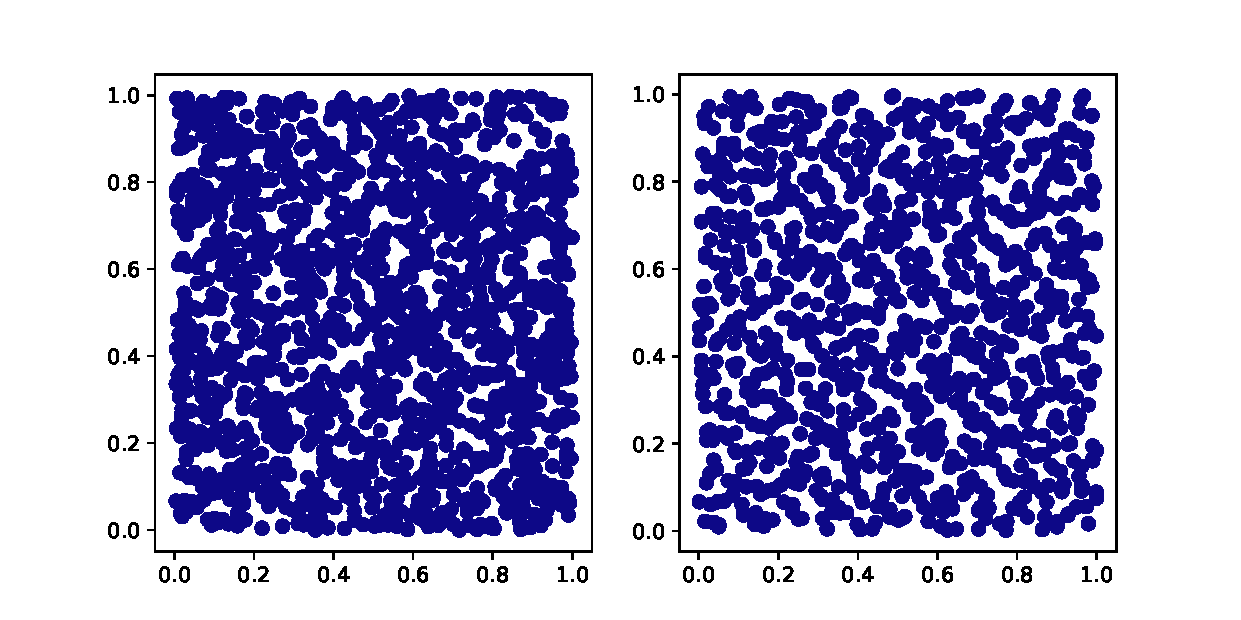
\includegraphics[width=\linewidth]{images/sampling.pdf}
    \caption{Наборы точек из двумерного пространства, взятые из равномерного случайного распределения (слева) и последовательности псевдослучайных чисел Соболя (справа)}
\end{figure}

\item Столбцы матрицы $C_i$ есть столбцы $B$ за исключением iго, который берется из $A$:
\begin{displaymath}
C_i=\begin{bmatrix}
x_{k+1}^{(1)} & x_{k+2}^{(1)} & \ldots & x_i^{(1)} & \ldots & x_{2k}^{(1)} \\
x_{k+1}^{(2)} & x_{k+2}^{(2)} & \ldots & x_i^{(2)} & \ldots & x_{2k}^{(2)} \\
\ldots & \ldots & \ldots & \ldots & \ldots & \ldots \\
x_{k+1}^{(N-1)} & x_{k+2}^{(N-1)} & \ldots & x_i^{(N-1)} & \ldots & x_{2k}^{(N-1)} \\
x_{k+1}^{(N)} & x_{k+2}^{(N)} & \ldots & x_i^{(N)} & \ldots & x_{2k}^{(N)} \\
\end{bmatrix}.
\end{displaymath}
\item Вычисляется вывод модели при всех наборах параметров из матриц $A$, $B$, $C_i$, то есть получаются три вектора размерности $N\times 1$:
\begin{displaymath}
y_A=f(A)\qquad y_B=f(B) \qquad y_{C_i}=f(C_i).
\end{displaymath} 
\item Вычисляется индекс Соболя первого порядка
\begin{displaymath}
S_i=\frac{V[E(Y|X_i)]}{V(Y)}=\frac{y_A\cdot y_{C_i}-f_0^2}{y_A\cdot y_A -f_0^2}=\frac{(1/N)\sum_{j=1}^N y_A^{(j)}y_{C_i}^{(j)} - f_0^2}{(1/N)\sum_{j=1}^N (y_A^{(j)})^2 - f_0^2},
\end{displaymath}
где
\begin{displaymath}
f_0^2=\left(\frac{1}{N}\sum\limits_{j=1}^N y_A^{(j)}\right)^2.
\end{displaymath}

Аналогично полный индекс Соболя
\begin{displaymath}
S_{T_i}=1-\frac{V[E(Y|\bm{X}_{\sim i})]}{V(Y)}=1-\frac{y_B\cdot y_{C_i}-f_0^2}{y_A\cdot y_A -f_0^2}=1-\frac{(1/N)\sum_{j=1}^N y_B^{(j)}y_{C_i}^{(j)} - f_0^2}{(1/N)\sum_{j=1}^N (y_A^{(j)})^2 - f_0^2}.
\end{displaymath}
\end{itemize}

Преимуществом такого подхода является тот факт, что для вычисления индексов по $k$ параметрам требуется только $N(k+2)$ запусков симуляции в отличие от полного перебора $N^2$ точек пространства параметров. Метод позволяет вычислить только полные индексы и индексы первого порядка, но они являются самыми информативными, поэтому мы ограничимся ими в данной работе \cite{saltelli2008global}.


\subsection{Исследуемая агентная модель}
\section{Результаты}
\subsection{Город и сателлиты}

\begin{figure}[H]
    \centering
    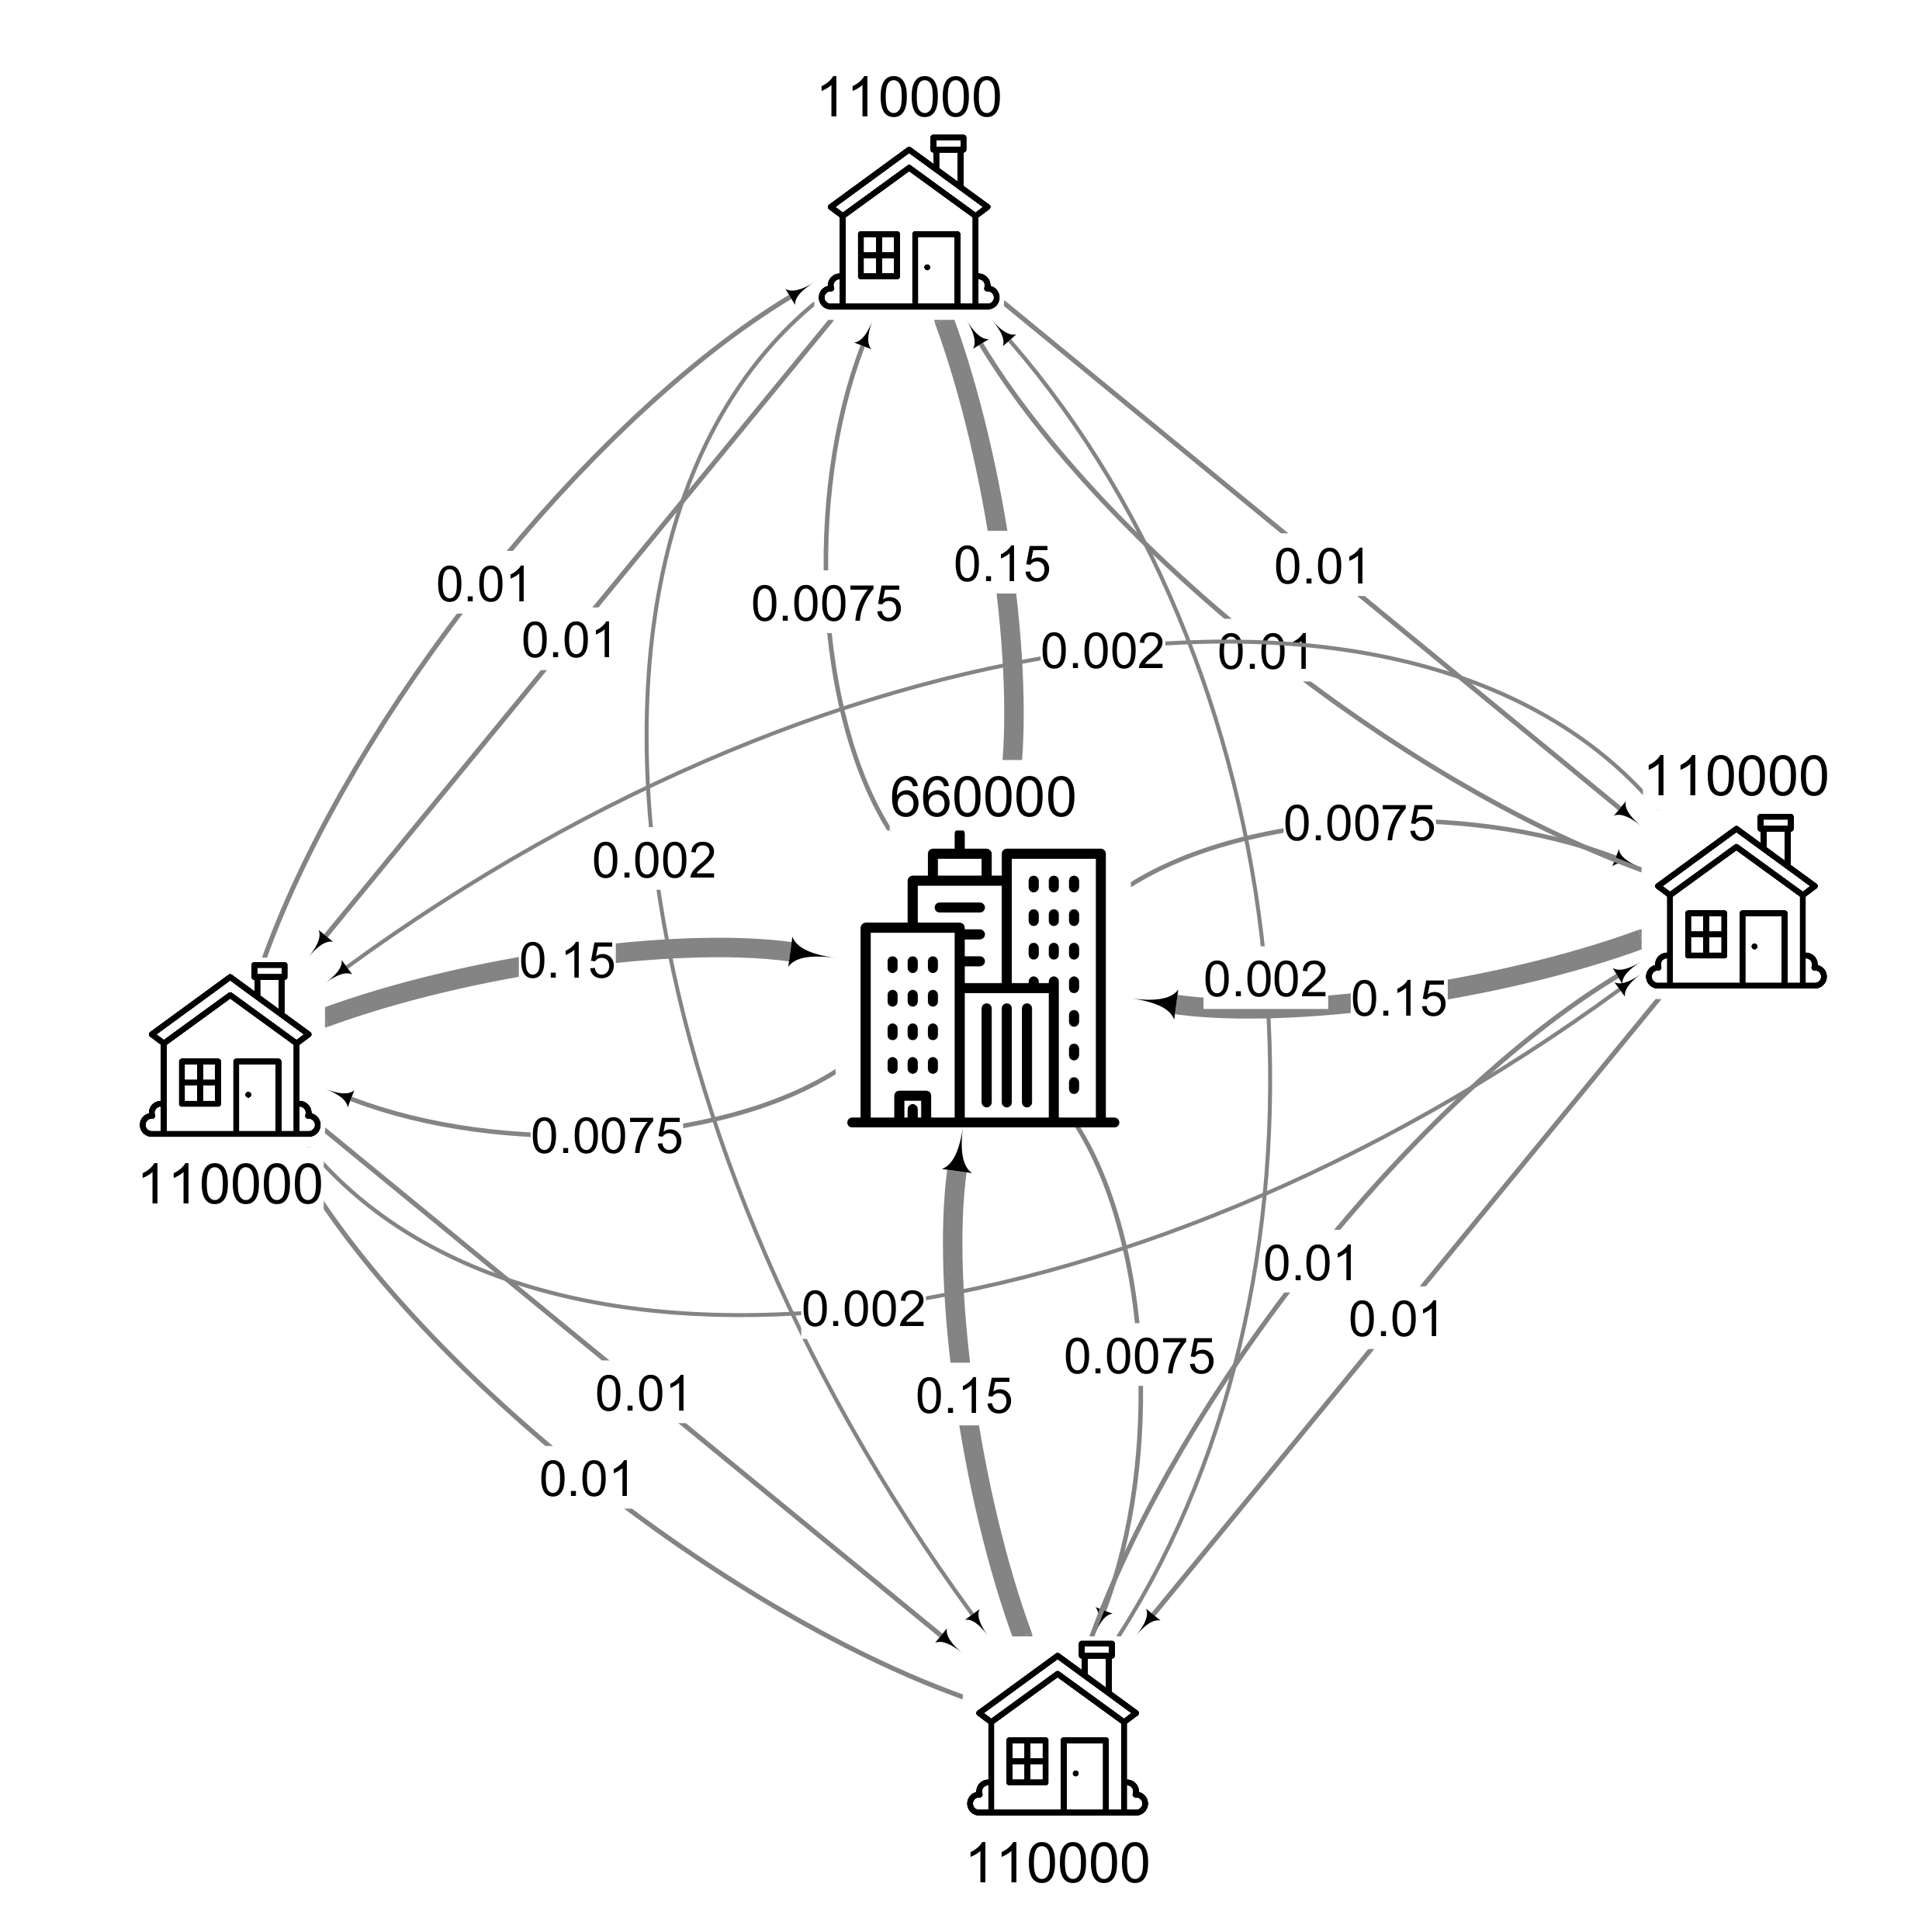
\includegraphics[width=0.4\linewidth]{images/graph1.png}
    \caption{Представление рассматриваемой модели транспортных потоков в системе большой город и сателлиты в виде графа (слева).}
\end{figure}

\begin{figure}[H]
    \centering
    \begin{subfigure}{0.45\linewidth}
        \centering
        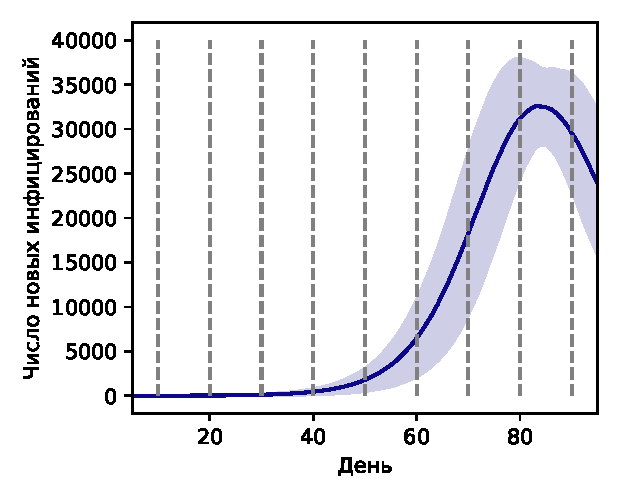
\includegraphics[width=\linewidth]{images/satellites_epid0.pdf}
    \end{subfigure}
    \hfill
    \begin{subfigure}{0.45\linewidth}
        \centering
        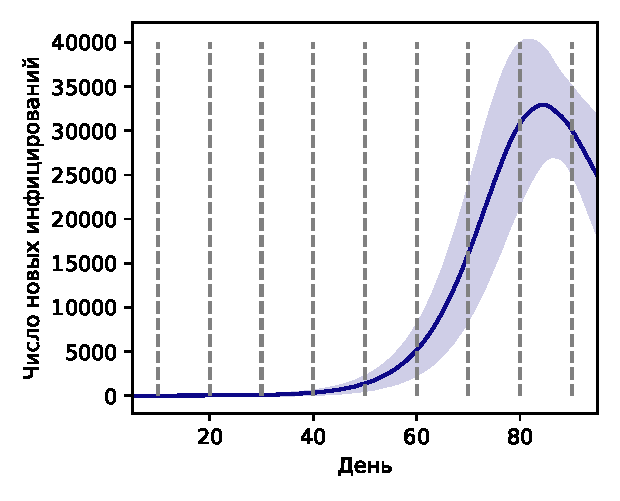
\includegraphics[width=\linewidth]{images/satellites_epid1.pdf}
    \end{subfigure}
    \caption{Суммарное число новых ежедневных инфицирований в системе при моделировании в отсутствие ограничительных мер при начале эпидемии в большом городе (слева) и в сателлите (справа).}
\end{figure}

\begin{figure}[H]
    \centering
    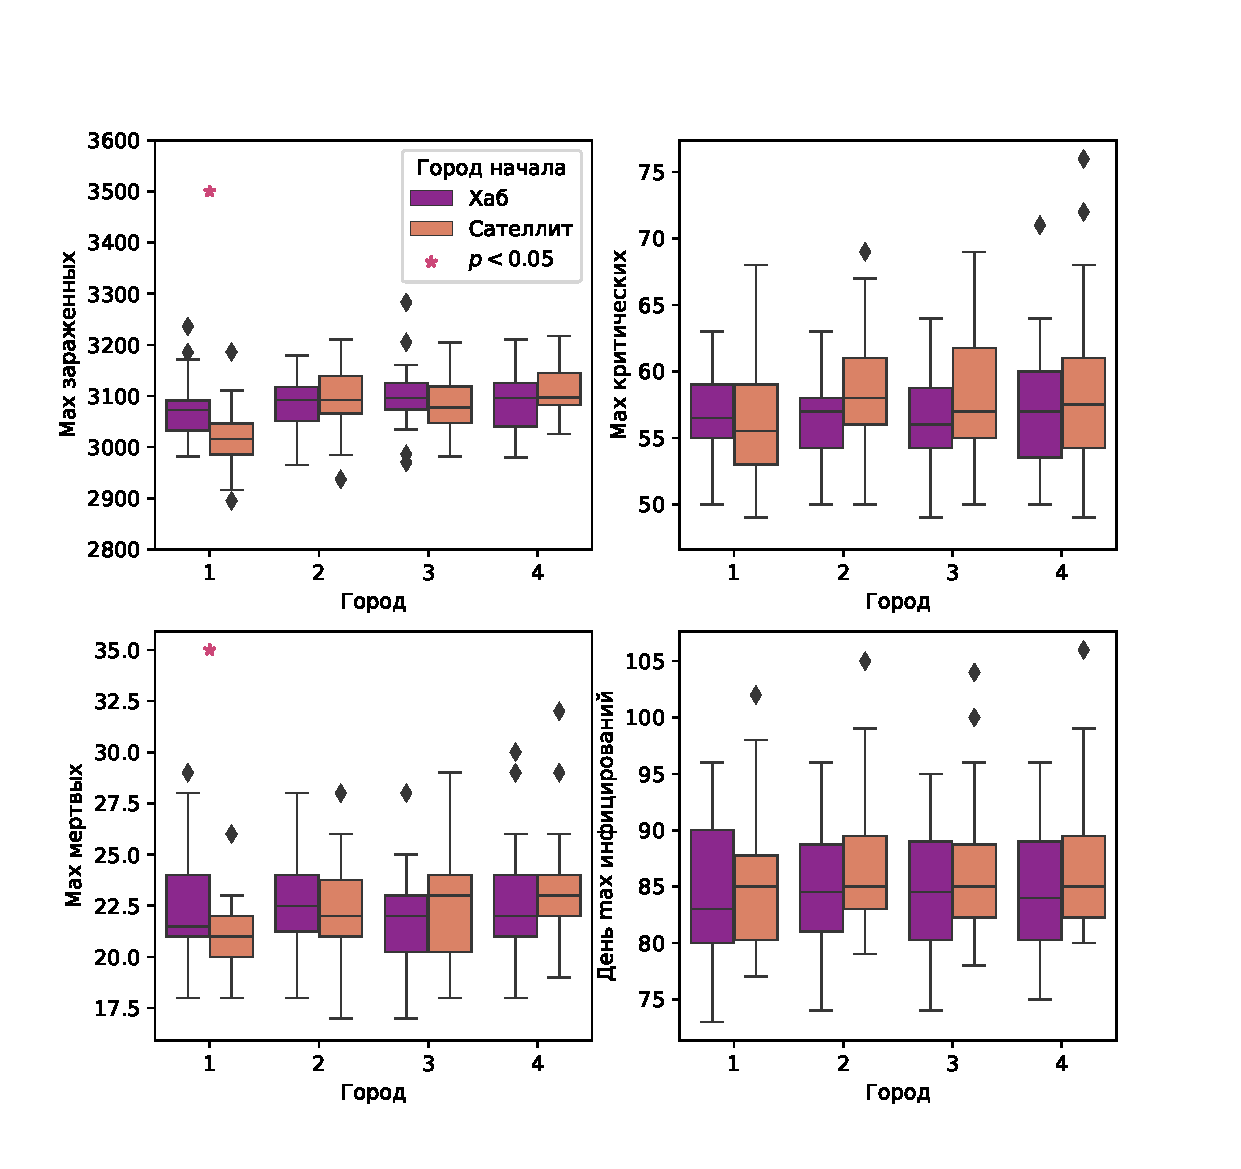
\includegraphics[width=\linewidth]{images/satellites_boxs.pdf}
    \caption{Исследуемые метрики в различных городах системы в зависимости от места начала эпидемии (ограничительные меры отсутствуют)}
\end{figure}

\begin{figure}[H]
    \centering
    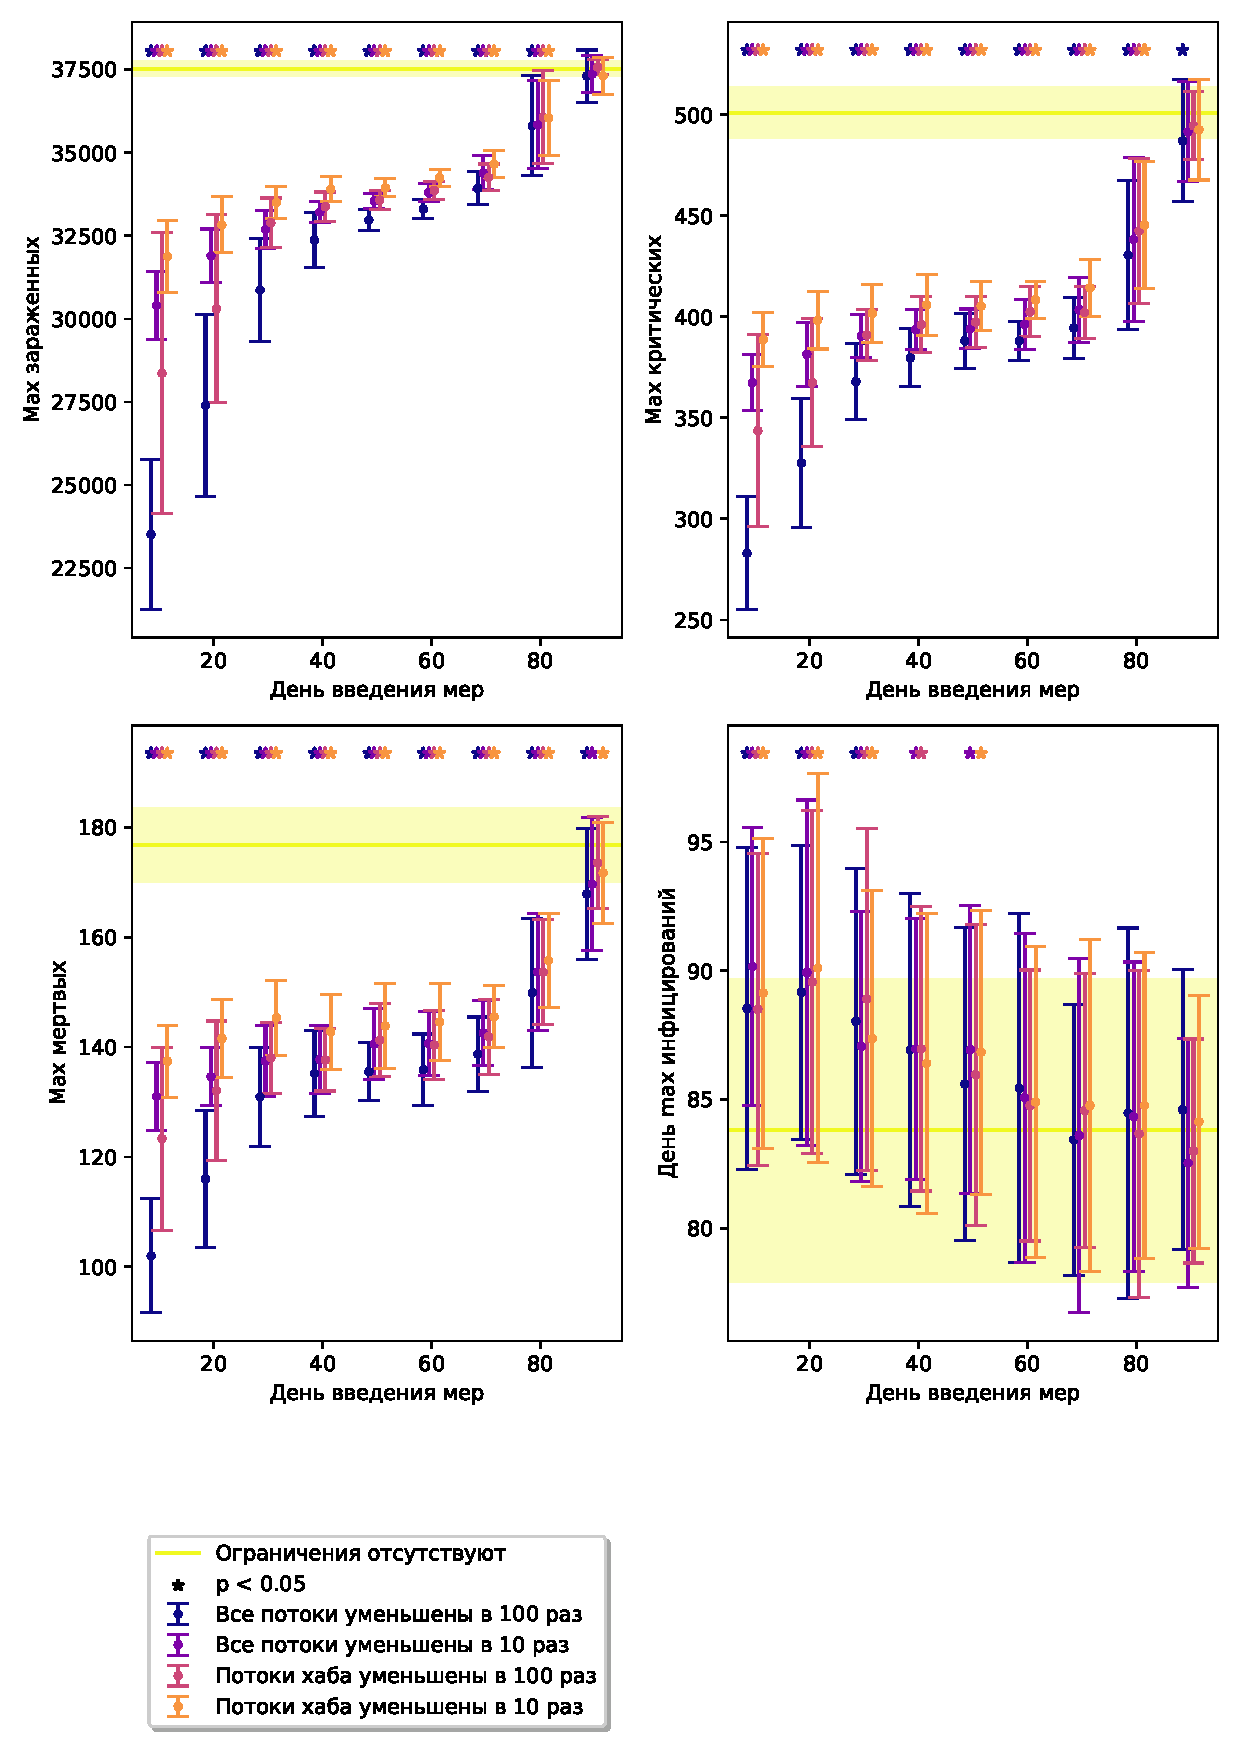
\includegraphics[width=\linewidth]{images/satellites_hists0.pdf}
    \caption{Зависимости исследуемых метрик системы от дня введения ограничений на транспортные потоки и величины этих ограничений при начале эпидемии в центральном городе.}
\end{figure}

\begin{figure}[H]
    \centering
    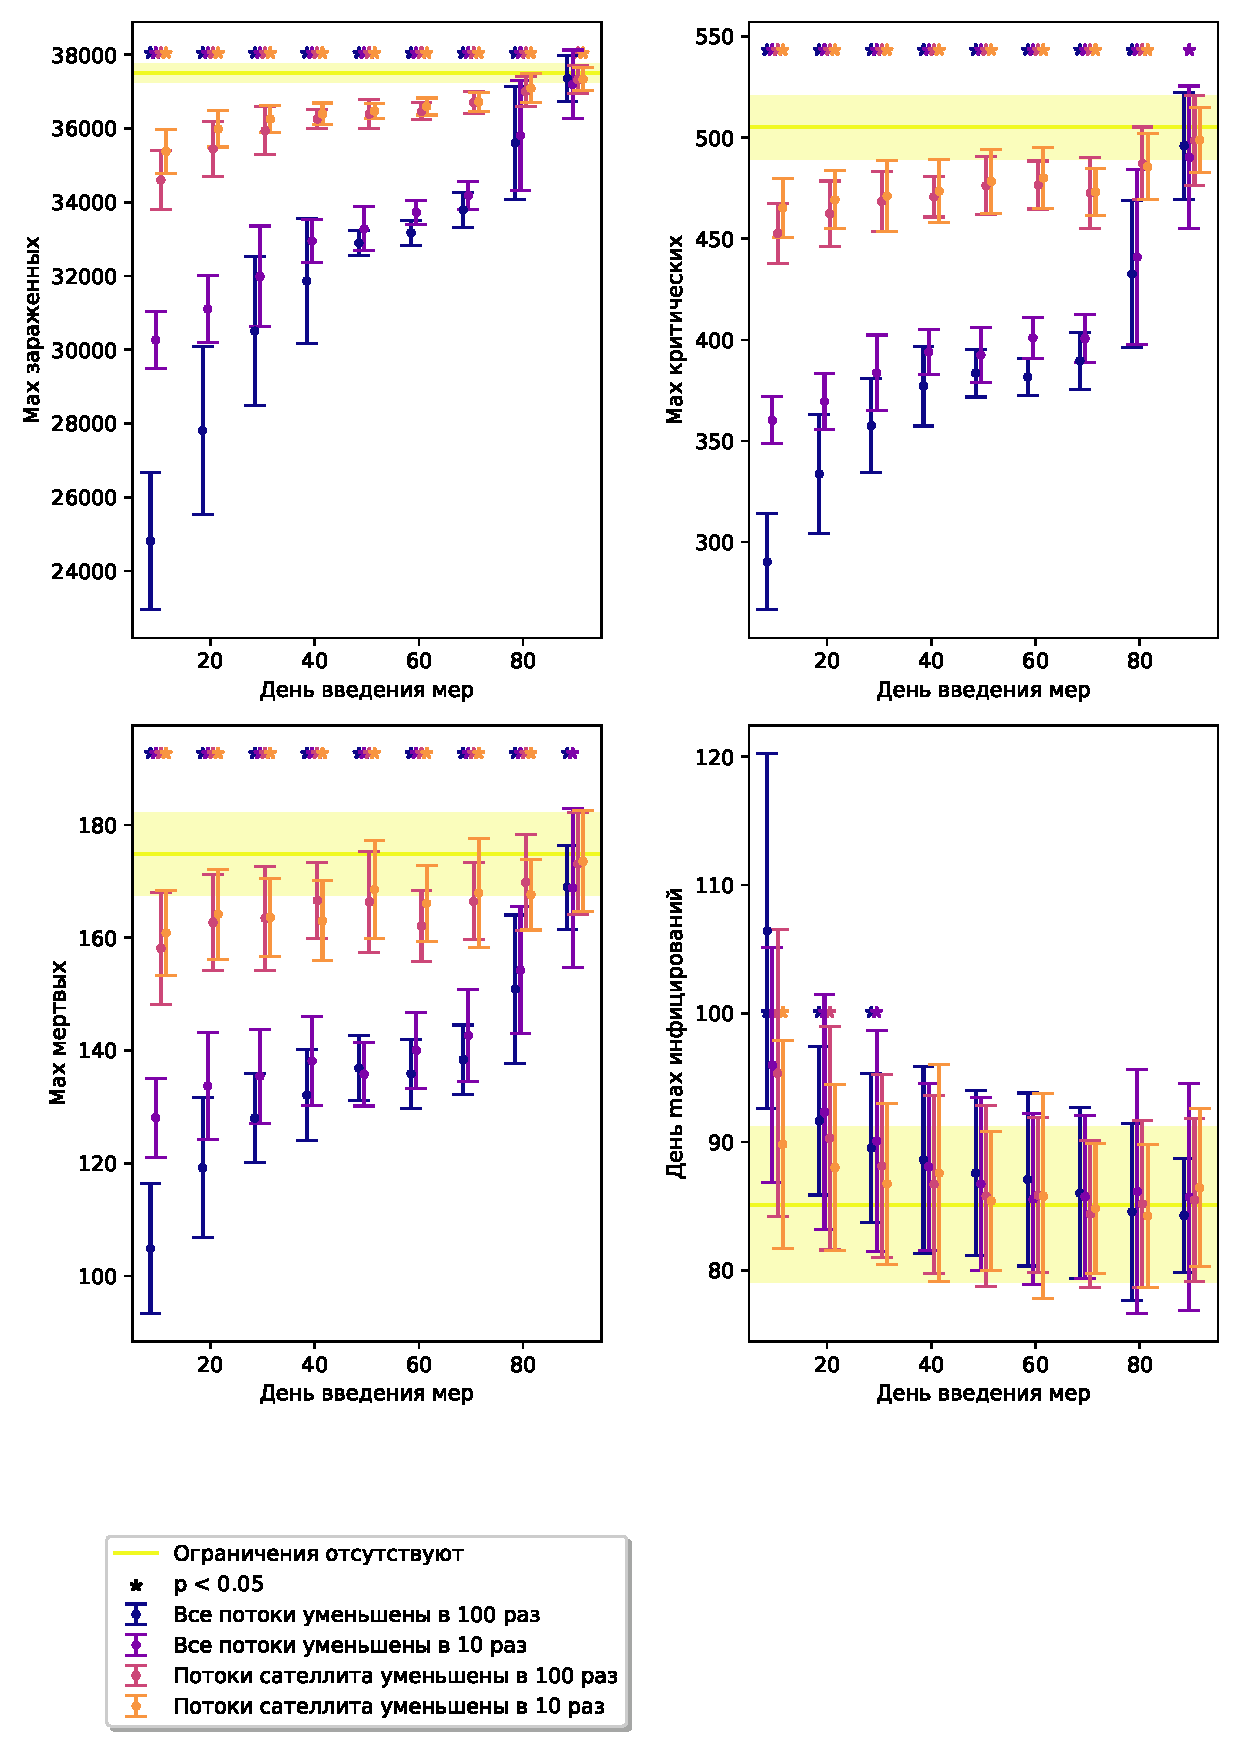
\includegraphics[width=\linewidth]{images/satellites_hists1.pdf}
    \caption{Зависимости исследуемых метрик системы от дня введения ограничений на транспортные потоки и величины этих ограничений при начале эпидемии в городе-сателлите.}
\end{figure}

\cite{makhrova2017work}

\subsection{Базовые потоки}

\begin{figure}[H]
    \centering
    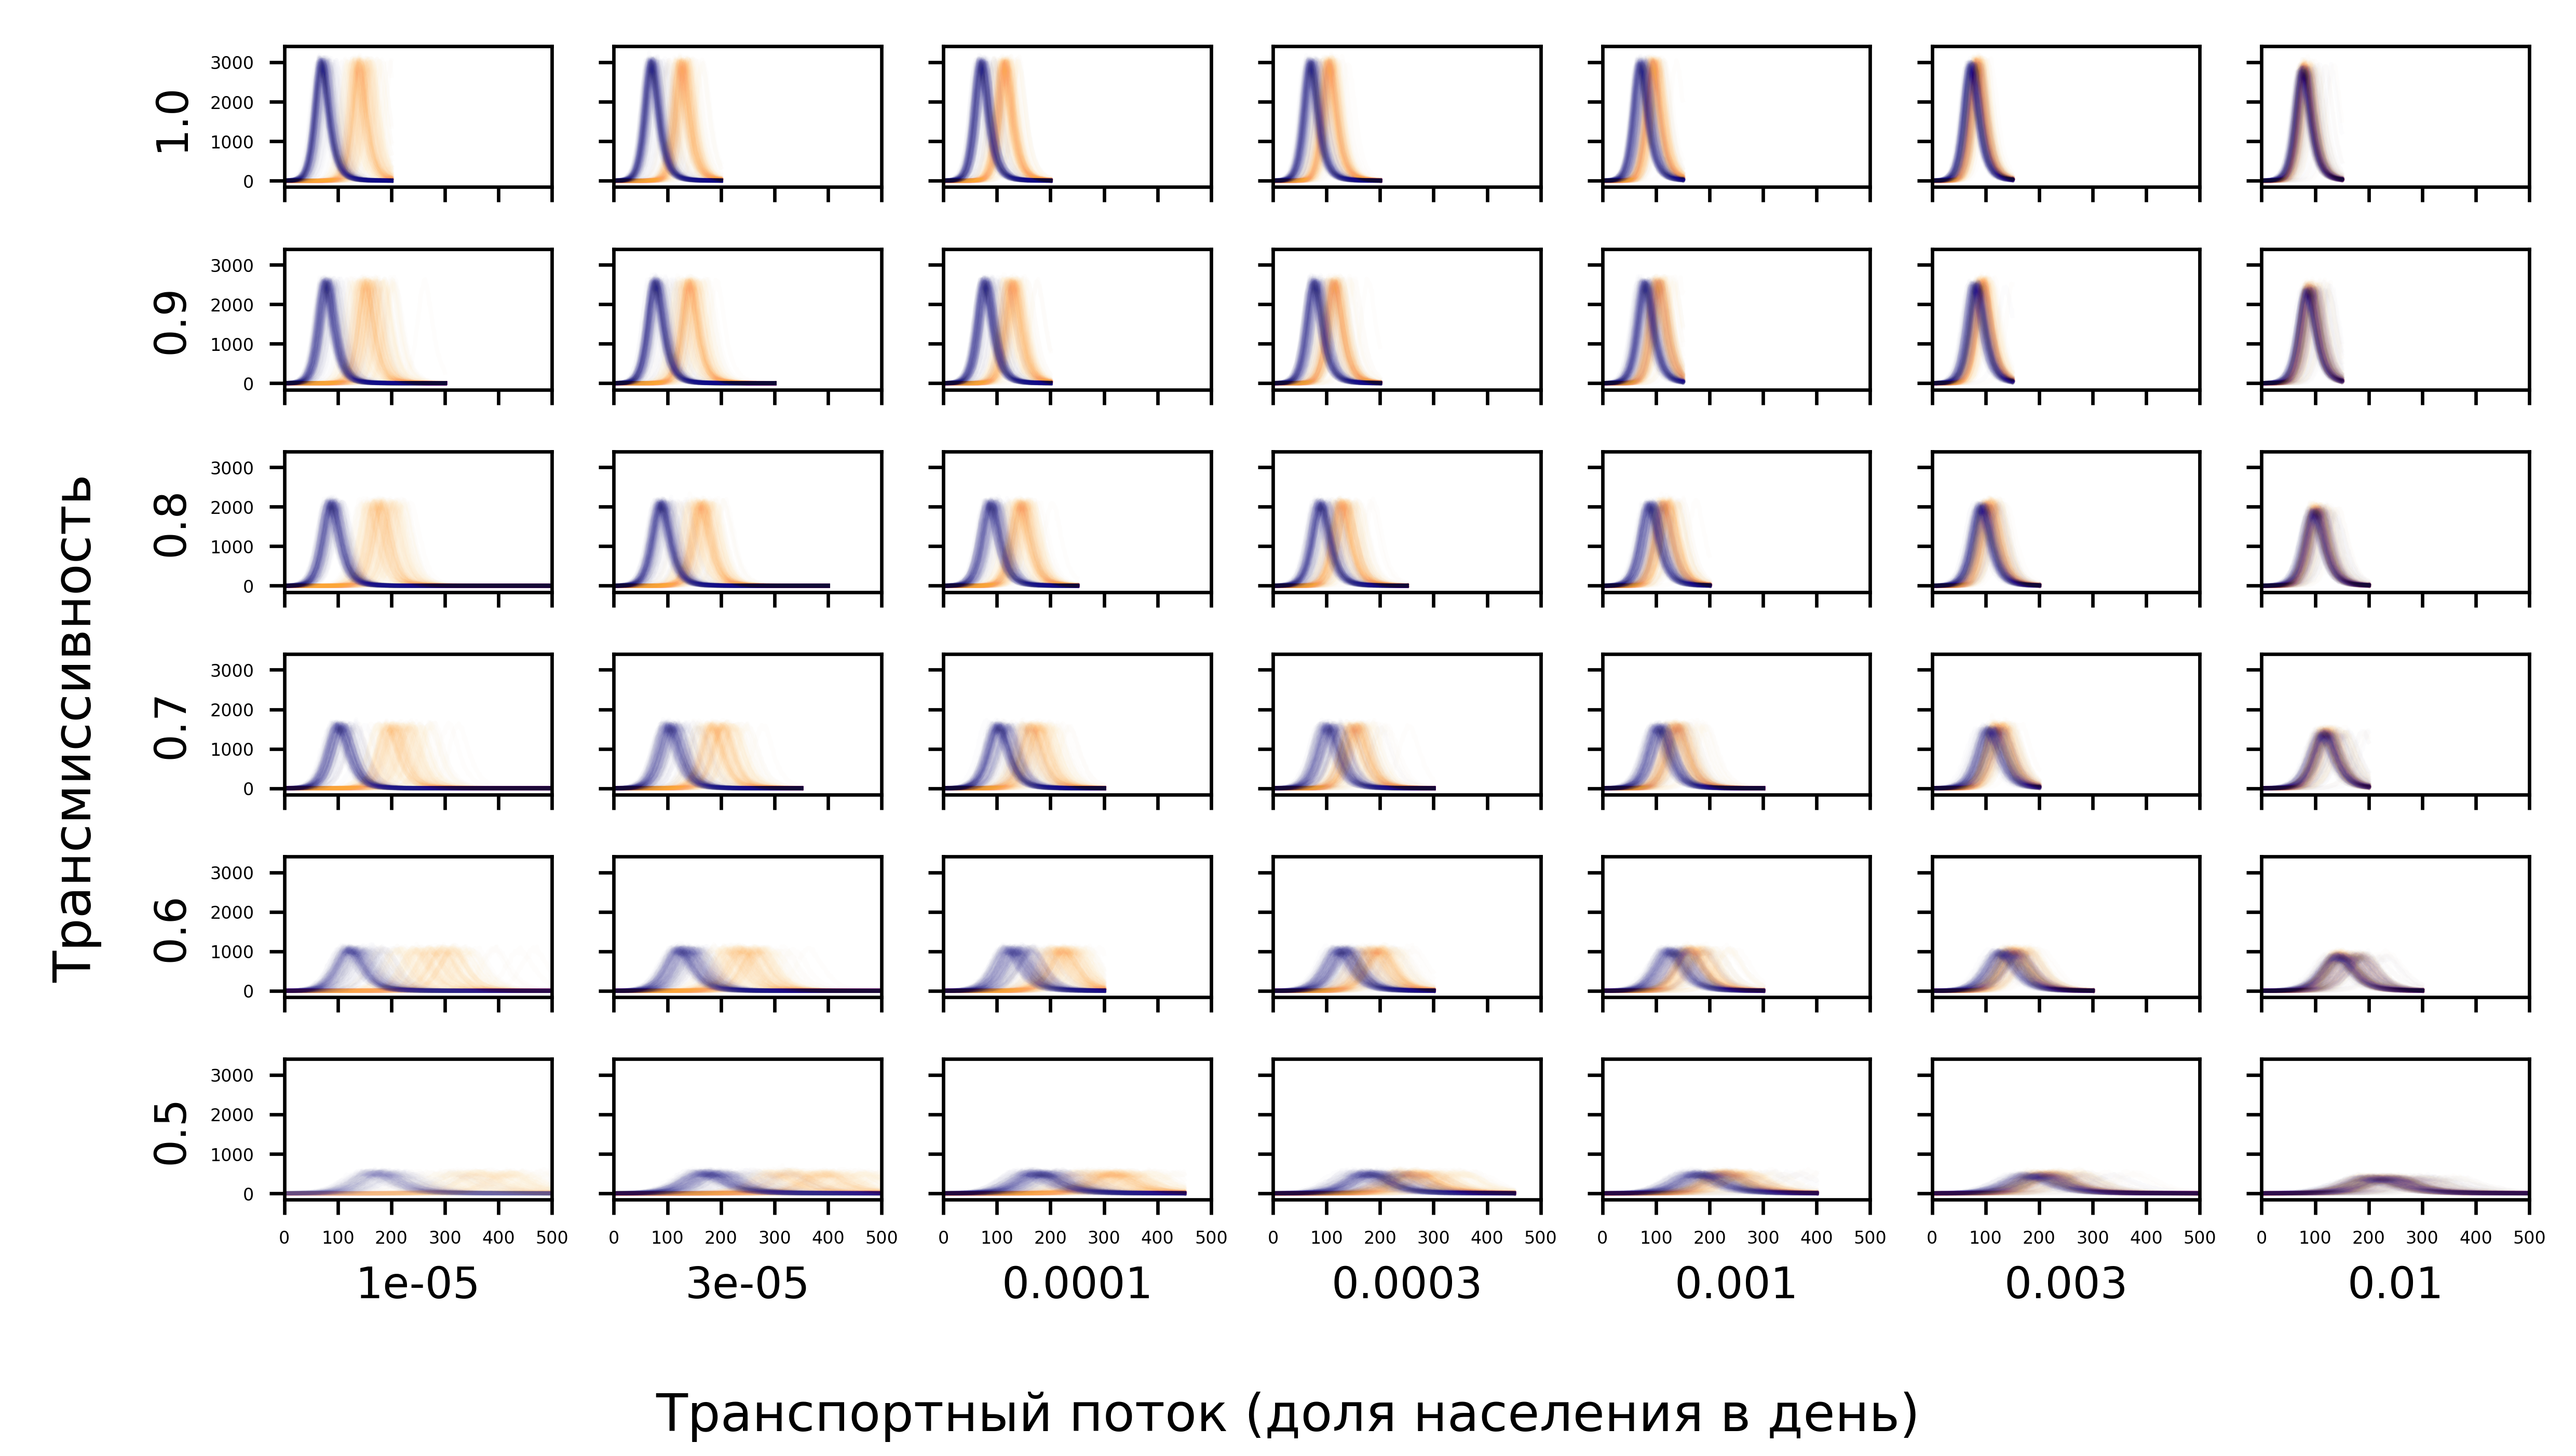
\includegraphics[width=\linewidth]{images/flows_epids_lines.pdf}
    \caption{Эпидемиологические кривые по результатам моделирования двух городов при разных трансмиссивностях инфекции и пассажиропотоках (на каждом графике 150 экспериментов).}
\end{figure}

\begin{figure}[H]
    \centering
    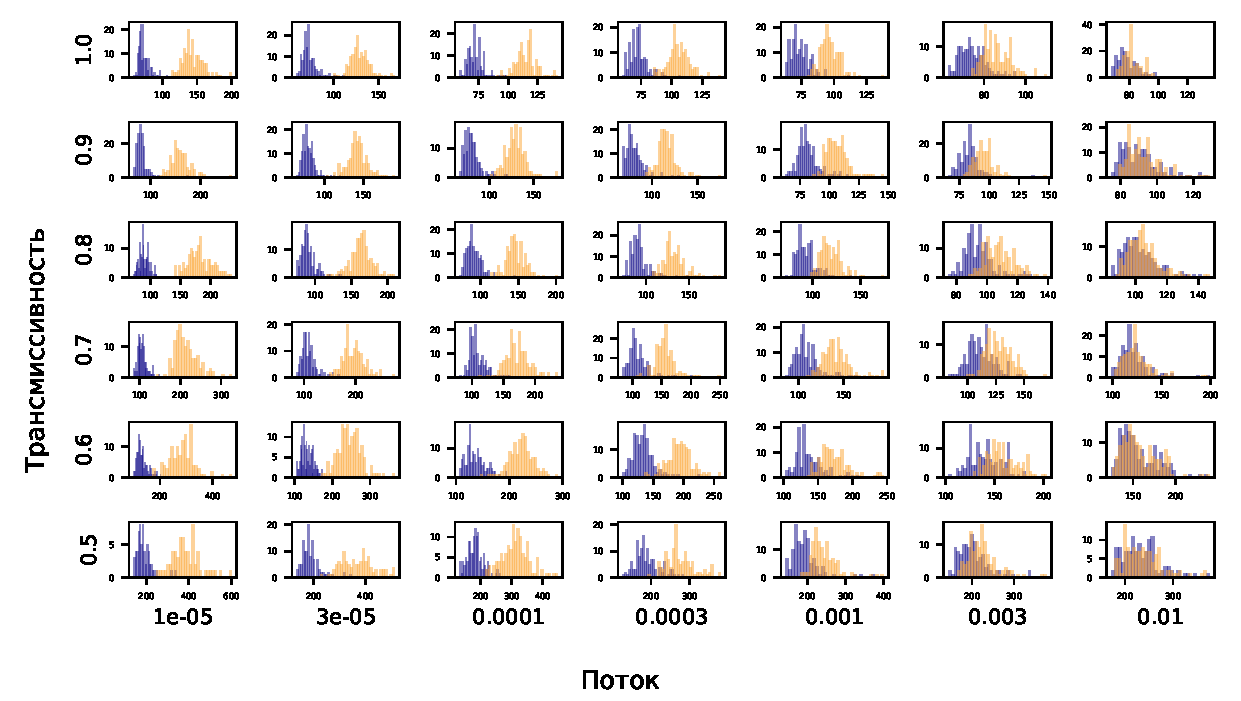
\includegraphics[width=\linewidth]{images/flows_hists_day.pdf}
    \caption{Гистограммы распределения дня пика инфицирований для двух городов (синяя соответствует городу начала эпидемии, оранжевая --- второму городу).}
\end{figure}

\begin{figure}[H]
    \centering
    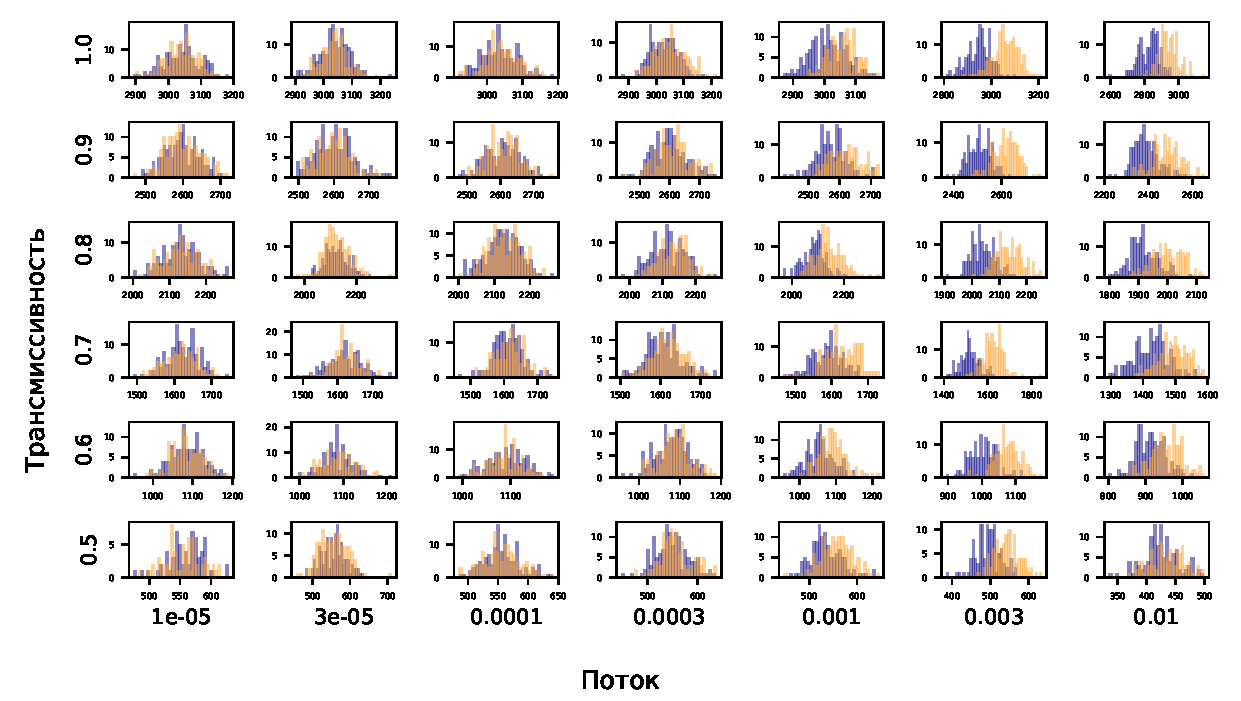
\includegraphics[width=\linewidth]{images/flows_hists_infs.pdf}
    \caption{Гистограммы распределения пикового числа инфицирований для двух городов (синяя соответствует городу начала эпидемии, оранжевая --- второму городу).}
\end{figure}

\begin{figure}[H]
    \centering
    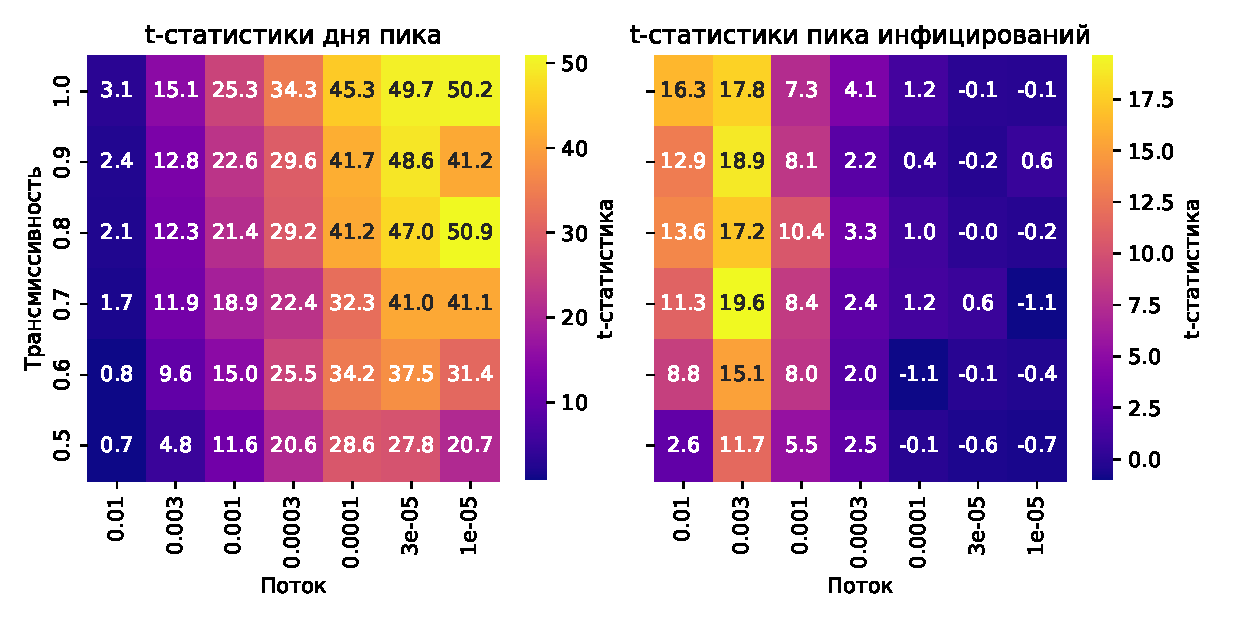
\includegraphics[width=\linewidth]{images/flows_heatmap_thesis.pdf}
    \caption{Тепловые карты t-статистик при сравнении метрик для двух городов (слева --- день пика инфицирований, справа --- пиковое число инфицирований).}
\end{figure}

\subsection{Индексы Соболя}

\begin{figure}[H]
    \centering
    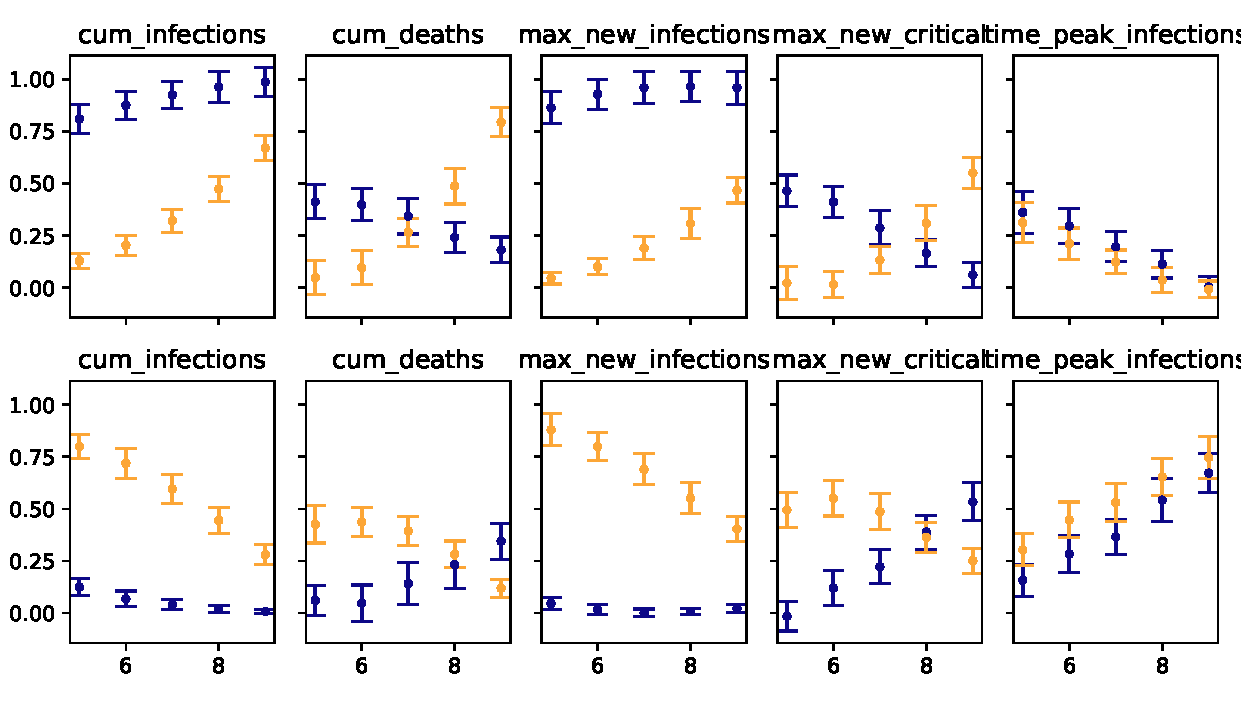
\includegraphics[width=\linewidth]{images/flow_to_small_S1_index.pdf}
    \caption{}
\end{figure}

\section{Выводы}
\section{Благодарности}
\section{Список литературы}


\printbibliography

\end{document}
